%!TEX program = pdflatex
% Full chain: pdflatex -> bibtex -> pdflatex -> pdflatex
\RequirePackage{etex}
\documentclass[11pt,en,authoryear]{elegantpaper}
%--------------------add packages----------------------%
%--------------------algorithm----------------------%
\usepackage{algorithm}
\usepackage{algpseudocode}
\usepackage{amsmath}
\usepackage{graphicx}
\usepackage{subfigure}
\usepackage{hyperref}
\renewcommand{\algorithmicrequire}{\textbf{Input:}}  % Use Input in the format of Algorithm
\renewcommand{\algorithmicensure}{\textbf{Output:}} % Use Output in the format of Algorithm
\numberwithin{equation}{section}

\newcommand{\HRule}{\rule{\linewidth}{0.5mm}} 
\newcommand{\told}{\text {old }}
\newcommand{\tnew}{\text {new }}
\newcommand{\mbR}{\mathbb{R}}
\newcommand{\mS}{\mathcal{S}}
\title{One-shot Distributed Lasso Regression}
\author{Zhe Li \\ Fudan University}
\institute{\href{https://sds.fudan.edu.cn/}{School of Data Science}}

%\version{0.08}
\date{\today}

\lstset{ 
  showstringspaces=false
}
\AtBeginEnvironment{lstlisting}{\linespread{1}\selectfont}

\begin{document}
\setlength{\belowcaptionskip}{-1cm} 

\begin{titlepage}
\begin{center}
% Upper part of the page
\textsc{\LARGE Fudan University}\\[1.5cm]
\textsc{\Large DATA620008: \ Optimization Theory}\\[0.5cm]
% Title
\HRule \\[0.6cm]
{ \huge \bfseries Final Project: }\\[0.4cm]
{ \huge \bfseries One-shot Distributed Lasso Regression}\\[0.4cm]

\HRule \\[1.5cm]

\includegraphics[width=2in]{logo.jpg}\\[1cm]

% Author
\begin{minipage}{0.4\textwidth}
\begin{flushleft} \large


\begin{center}
\vspace{0.5cm}
\textbf{Author}\\
\vspace{0.4cm}
Zhe Li \hspace*{0.8cm} 20210980134\\
\end{center}
\end{flushleft}
\end{minipage}
\vfill
% Bottom of the page
{\large \today}
\end{center}
\end{titlepage}

\tableofcontents

\newpage

\maketitle


\begin{abstract}
In this work, we develop a distributed lasso regression approximation (\textbf{DLR}) method that is able to solve the lasso regression problem on a distributed system. 
To handle the problem, we distribute the dataset on different worker servers.
An traditional optimization algorithm (PGM, ADMM, Subgradient descent) is first conducted on each worker to get the local estimator. 
After that, the informations on each worker are then broadcasted to master to obtain a combined estimator by taking a weighted average of local estimators. The proposed distributed algorithm has three merits. 
First, the communication cost is low since it requires only one round of communication. Second, no further iterative algorithm is needed on master and hence it does not suffer from problems as initialization and non-robustness. Third, the computational complexity is much lower compared to get the global estimator using whole dataset. The code of the project can be found in ({\href{www.github.com/Ikerlz/dlra}{www.github.com/Ikerlz/DLR}}). Theoretical properties are provided with respect to the estimation consistency. Lastly, the advantages of the proposed methodology are illustrated by experiments on a variety of synthetic and empirical datasets.
\keywords{Lasso; Distributed system; Optimization algorithm}
\end{abstract}

\section{INTRODUCTION}

Data Analysis with huge datasets has become more and more popular in today’s world. Consequently, the dataset must be stored and processed on many connected computer nodes, which thereafter are referred to as a distributed system \citep{zhu2019least}. Furthermore, A distributed system is a system with multiple components located on different machines that communicate and coordinate actions in order to appear as a single coherent system to the end-user.

In this work, we consider a \textbf{“master-and-worker”}-type distributed system with strong workers. As one will see, the most widely used systems, Hadoop \citep{hadoop2011apache} and Spark \citep{spark2018apache}, belong to this category. In this systems architecture, the workers is mainly responsible for the computation task and do not communicate with each other directly. In constract, the master should communicate with each worker and collect all the information from workers to get the final result. Since the communication cost between the master and workers is expensive, we should try to consider “one-shot” (OS) approach first, which requires only one round of communication. Specifically, the local worker computes the estimators in parallel and then communicate to the master to obtain an average global estimator \citep{zhang2012communication,liu2014distributed,chang2017distributed,fan2019distributed}. However "one-shot" algorithms may not achieve the best efficiency in statistical estimation in most occasions since there is not enough communications between master and workers \citep{smith2018cocoa}. Therefore, developing algorithms that are highly efficient computationally, communicationally and statistically for distributed systems has become a problem of great interest.

The aforementioned approach is also studied for the regression problem using $\ell_1$ shrinkage estimation (i.e. Lasso Regression). 
\citep{battey2015distributed} use the MapReduce structure to solve the lasso problem and further considered distributed testing and estimation methods in a unified likelihood framework, in which a refitted estimation is used to obtain an oracle convergence rate. For the second approach, both \citep{wang2017efficient} and \citep{jordan2018communication} have developed iterative algorithms to solve the sparse estimation problem, and they theoretically proved that the error bounds match the centralized estimator. Beyond the $\ell_1$ shrinkage estimation, \citep{chen2014split} studied a penalized likelihood estimator with more general penalty function forms in a high-dimensional setting. However, to the best of our knowledge, all of the above methods assume independent and identical samples stored by each worker, which is questionable in practice because the distributed dataset might experience great heterogeneity from worker to worker.

In this work, we aim to develop a novel methodology to address the Lasso regression. Specifically, we assume the data possessed by different workers are allowed to be heterogeneous but share the same regression relationship. The proposed method borrows the idea of the distributed least squares approximation, i.e. DLSA \citep{zhu2019least} and can be used to handle a large class of parametric regression models on a distributed system. Specifically, let $Y \in \mathbb{R}$ be the response of interest, let $X$ be the associated predictor, and let $\theta \in \mathbb{R}^p$ be the corresponding regression coefficient. The objective is to estimate the regression parameter $\theta$ using lasso regression on a distributed system that has one master and many strong workers. Under this setting, we propose a distributed Lasso regression (DLR) method. The key idea is as follows:

\begin{itemize}
    \item First, we estimate the parameter $\theta$ on each worker separately by using local data on distributed workers. This can be done efficiently by using standard optimization methods (e.g., Subgradient descent, proximal gradient descent, ADMM). By assuming that the sample size of each worker is sufficiently large, the resulting estimator and its asymptotic covariance estimate should be consistent but not statistically efficient, as compared with the global estimates.
    \item Next, each worker passes the local estimator of $\theta$ and its asymptotic covariance estimate (a $p \times p$ matrix) to the master.
    \item Once the master receives all the local estimators from the workers, a weighted least squares-type objective function can be constructed. This can be viewed as a local quadratic approximation of the global log-likelihood functions. As one can expect, the resulting estimator shares the same asymptotic covariance with the full-size MLE method (i.e., the global estimator) under appropriate regularity conditions.
\end{itemize}

\begin{center}
    \begin{figure}[h]
        \centering
        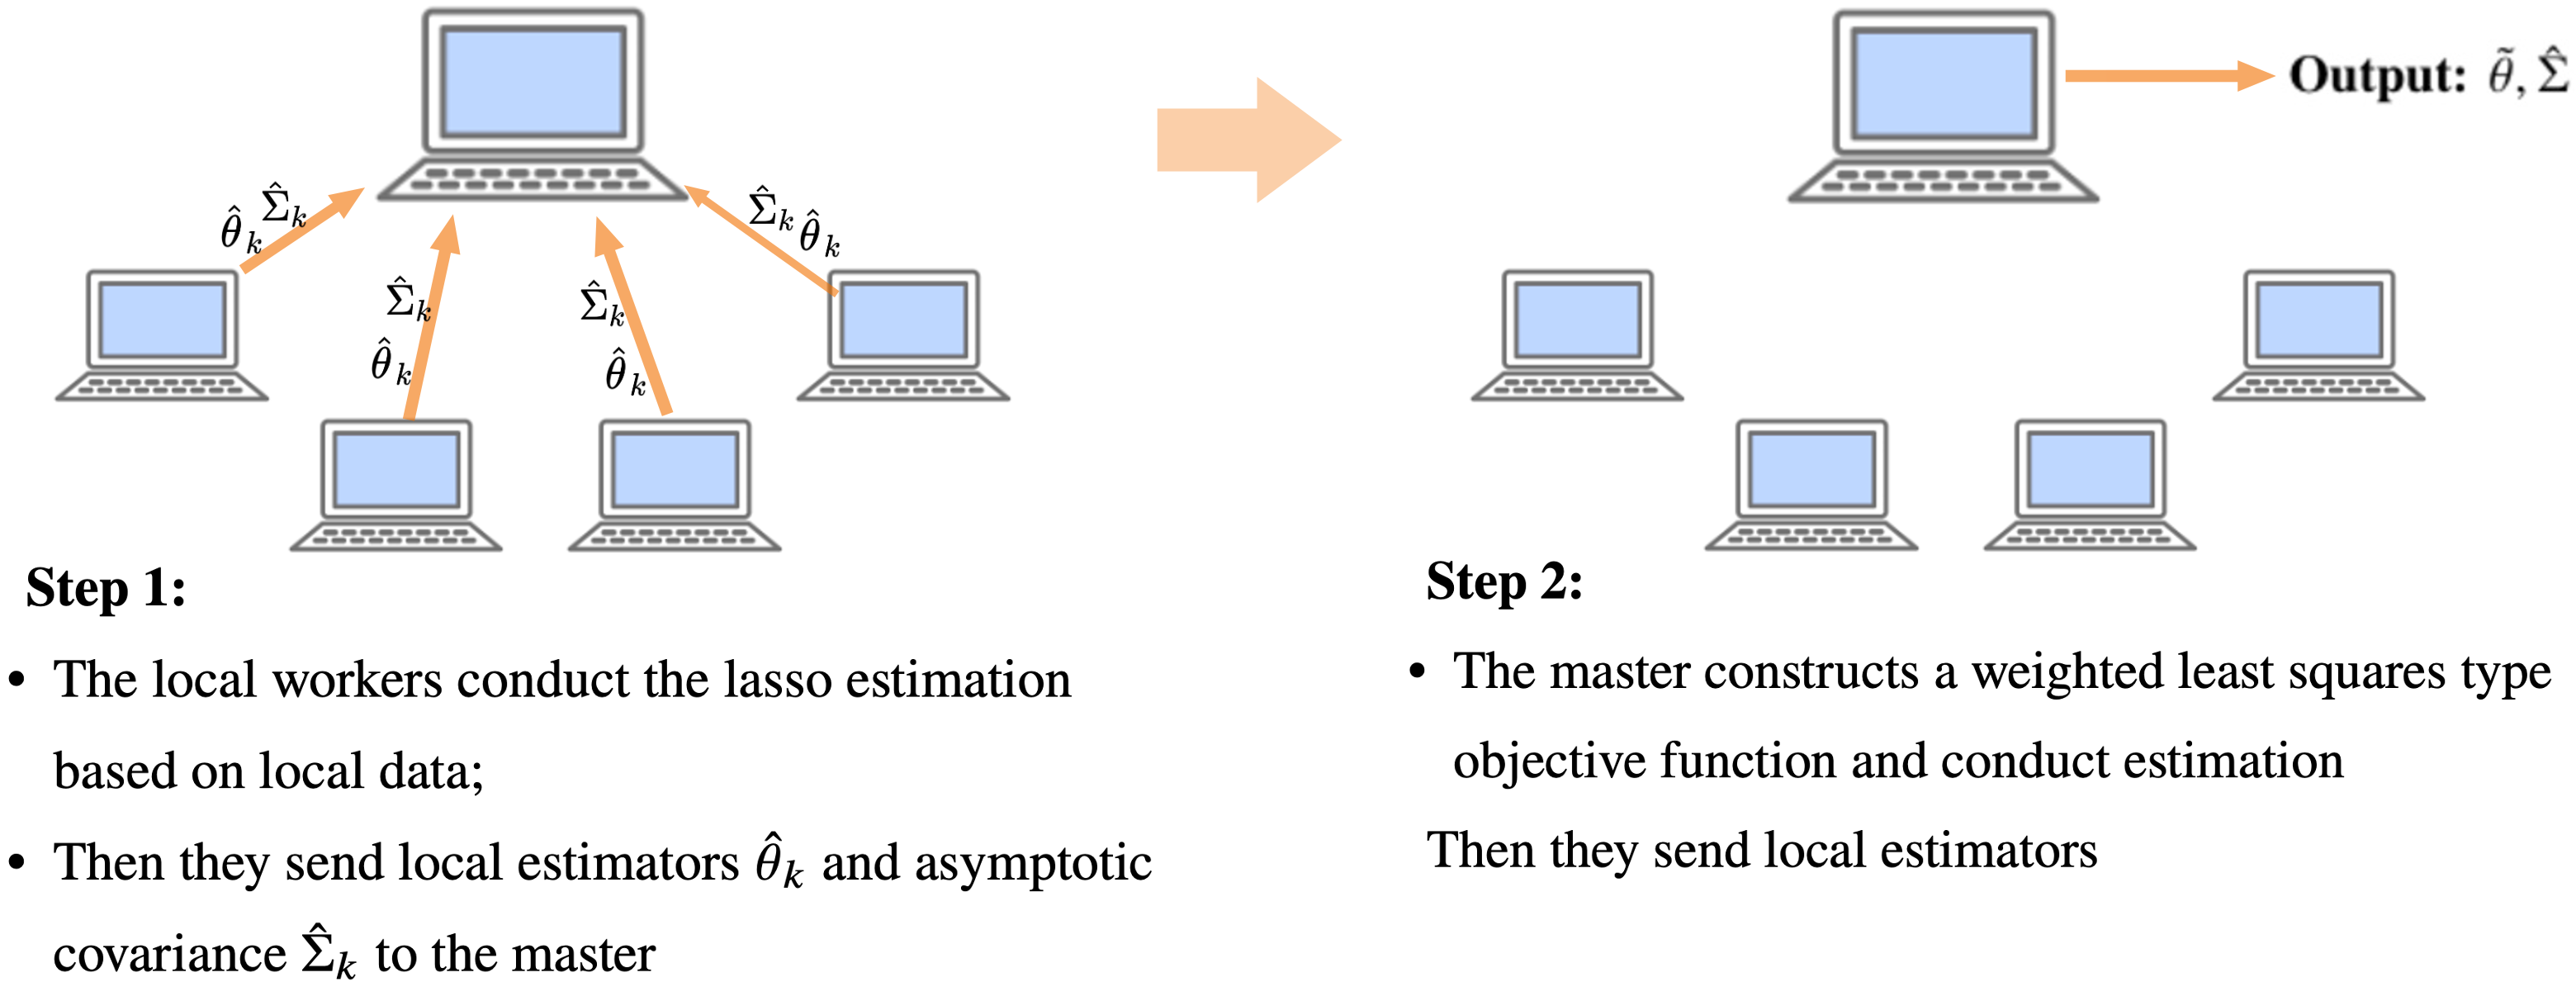
\includegraphics[width=0.7\textwidth]{image/fig1.png}
        \caption{Illustration of the DLR method.}
        \label{fig1}
    \end{figure}
\end{center}

The major steps of the DLR method are further illustrated in Figure \ref{fig1} and 
the remainder of this article is organized as follows. Section \ref{sec:2} introduces the model setting and the distributed lasso regression algorithm. We develop the theoretical properties of the estimation in Section \ref{sec:3}. In Section \ref{sec:4} and \ref{sec:5}, we study the performance of our algorithm via simulation and real data analysis. Section \ref{sec:6} concludes the article with a discussion.
\section{DISTRIBUTED LASSO REGRESSION}\label{sec:2}

\subsection{Lasso Regression Model}\label{section:lasso_reg_model}

LASSO is actually an abbreviation for “Least absolute shrinkage and selection operator”, which was firstly proposed by \cite{tibshirani1996regression}. Consider there are in total $N$ observations, which are indexed as $i = 1,\ldots,N$. The $i$th observation is denoted as $Z_i = (X_i^{\top},y_i)^{\top} \in \mathbb{R}^{p+1}$, where $y_i \in \mathbb{R}$ is the response of interest and $X_i \in \mathbb{R}^p$ is the corresponding covariate vector. If we denote the parameter $\beta = (\beta_1, \beta_2, \ldots, \beta_p)^{\top} \in \mathbb{R}^{p}$, then the goal of Lasso is to get the estimation of $\beta$ (i.e. $\hat{\beta}^{L}$), which satisfies

\begin{equation}\label{equ:lasso}
    \hat{\beta}^{L}=\arg \min \frac{1}{2 N} \sum_{i=1}^{N}\left(y_{i}-X_i \beta\right)^{2}, \quad \text { s.t } \sum_{j=1}^{p}\left|\beta_{j}\right| \leq t
\end{equation}
Therefore, the lasso regression model could be written as 

\begin{equation}\label{equ:lasso_reg}
    y = X \beta + \lambda \|\beta \|_1
\end{equation}
where $y \in \mbR^{N}$, $X \in \mbR^{N \times p}$ and $\beta \in \mbR^{p}$. The shrinkage parameter $\lambda$ controls the value range of the variables, which means the $\ell_1$-norm is a penalty term. Thus, we can provide the variable selection by changeing the value of $\lambda$ in lasso regression model.

There are many algorithms to solve the lasso regression, such as \textbf{LARS} \citep{efron2004least}, \textbf{Coordinate Descent} \citep{wu2008coordinate}. However, in this article, we use three optimization algorithms to solve the lasso regression.

\subsubsection{Proximal Gradient Descent}
Proximal gradient methods are a generalized form of projection used to solve non-differentiable convex optimization problems. we can rewrite  equation (\ref{equ:lasso_reg}) as an unconstrained optimization with the composite model:
\begin{equation}
    \min_{\beta} f(\beta)=g(\beta)+h(\beta)
\end{equation}
where $g(\beta) = \frac{1}{2N}\|y - X \beta\|_{2}^{2}$ and $h(\beta) = \lambda\| \beta\|_1$. Since $h(\beta)$ is closed and convex function, then we can define the proximal mapping as follows:

\begin{definition}\label{def:prox}
Suppose $h$ is a closed and convex function. The proximal mapping (prox-operator)
of $h$ is defined as
\begin{equation}
\operatorname{prox}_{h}(x)=\underset{u}{\operatorname{argmin}}(h(u)+\frac{1}{2}\|u-x\|^{2})
\end{equation}
\end{definition}
\noindent
Following the definition \ref{def:prox} and $g^{\prime}(\beta) = -\frac{1}{N}X^{\top}(y - X\beta)$, the updating equation can be written as 
\begin{equation}\label{equ:pgm_update}
    \begin{aligned}
    \beta_{k+1} &= \operatorname{prox}_{\alpha h}\left(\beta_k - \alpha \cdot g^{\prime}(\beta_k) \right) \\
    &= \operatorname{sign}(\beta_k - \alpha \cdot g^{\prime}(\beta_k)) \max \left\{|\beta_k - \alpha \cdot g^{\prime}(\beta_k)|-\alpha \lambda, 0\right\}
    \end{aligned}
\end{equation}
The Proximal Gradient Descent of Lasso regression is summarized in Algorithm \ref{algo:pgd_lasso}.

\begin{center}
\begin{minipage}{13.5cm}
	  \begin{algorithm}[H]
  \caption{Proximal gradient descent of Lasso regression.}\label{algo:pgd_lasso}
  \begin{algorithmic}[1]
    \Require
      Dataset $Z = (X, y) \in \mbR^{N \times (p+1)}$;the shrinkage parameter $\lambda$;  the step size $\alpha$ (using constant step size); tolerance $\epsilon$; initial point $\beta_0$
    \Ensure Estimation of $\beta$: $\hat{\beta}$
    \For {$k=0,1,2,\ldots$}
    {
    \State update $\beta_{k+1} = \operatorname{sign}(\beta_k - \alpha \cdot g^{\prime}(\beta_k)) \max \left\{|\beta_k - \alpha \cdot g^{\prime}(\beta_k)|-\alpha \lambda, 0\right\}$ \quad (\ref{equ:pgm_update})
    \If{$\|\beta_{k+1}-\beta_{k} \|_2 < \epsilon$}
    \State stop
    \EndIf
    }
    \EndFor
  \end{algorithmic}
\end{algorithm}
\end{minipage}
\end{center}



\subsubsection{Subgradient Descent}

The subgradient method is a simple algorithm for minimizing a nondifferentiable convex function \citep{boyd2003subgradient}. we can calculate the subgradient of the loss function (\ref{equ:whole_loss}) directly using the definition \ref{def:subgrad}.
\begin{equation}\label{equ:whole_loss}
    \mathcal{L}(\beta) = \frac{1}{2N} \left\|y - X^{\top}\beta \right\|_2^2 + \lambda \|\beta \|_1
\end{equation}

\begin{definition}\label{def:subgrad}
Suppose $f: \mbR^{n}\rightarrow \mbR$ is a real-valued function. The subdifferential $\partial f(x)$ of $f$ at $x$ is the set of all subgradients:
\begin{equation}
    \partial f(x)=\left\{g \mid g^{T}(y-x) \leq f(y)-f(x), \forall y \in \operatorname{dom}(f)\right\}
\end{equation}
\end{definition}
Since the $\operatorname{sign}(\beta) \in \partial \|\beta \|_1$, the descent direction of the subgradient descent algorithm can be calculated as equation (\ref{equ:sgd_update}) and the algorithm is summarized in Algorithm \ref{algo:sgd_lasso}.
\begin{equation}\label{equ:sgd_update}
    d^{k}=-\left(\frac{1}{N}X(X^{\top}\beta-y)+\lambda \cdot \operatorname{sign}(\beta)\right)
\end{equation}

\begin{center}
\begin{minipage}{13.5cm}
	  \begin{algorithm}[H]
  \caption{Subgradient descent of Lasso regression.}\label{algo:sgd_lasso}
  \begin{algorithmic}[1]
    \Require
      Dataset $Z = (X, y) \in \mbR^{N \times (p+1)}$;the shrinkage parameter $\lambda$;  the step size $\alpha$ (using constant step size); tolerance $\epsilon$; initial point $\beta_0$
    \Ensure Estimation of $\beta$: $\hat{\beta}$
    \For {$k=0,1,2,\ldots$}
    {
    \State update $d^{k+1} = -\left(\frac{1}{N}X(X^{\top}\beta_k-y)+\lambda \cdot \operatorname{sign}(\beta)\right)$ \quad (\ref{equ:sgd_update})
    \State update $\beta_{k+1}= \beta_k - \alpha \cdot d^{k+1}$
    \If{$\|\beta_{k+1}-\beta_{k} \|_2 < \epsilon$}
    \State stop
    \EndIf
    }
    \EndFor
  \end{algorithmic}
\end{algorithm}
\end{minipage}
\end{center}

\subsubsection{Alternating Direction Method of Multipliers}

ADMM is used to solve the linearly constrained convex problem. We can regard the lasso regression as
\begin{equation}\label{equ:admm_problem}
\min _{\beta, z} \frac{1}{2N}\|X^{\top}\beta-y\|_{2}^{2}+\mu\|z\|_{1}, \quad \text { s.t. } \quad \beta=z
\end{equation}
To solve the problem (\ref{equ:admm_problem}), the Lagrange multiplier $u$ is introduced to obtain the augmented Lagrange function (\ref{equ:lagrange_admm}). Therefore, we can use the dual ascent method to solve it.
\begin{equation}\label{equ:lagrange_admm}
L_{\rho}(\beta, z, u)=\frac{1}{2N}\|X^{\top} \beta-y\|_{2}^{2}+\lambda\|z\|_{1}+u^{\top}(\beta-z)+\frac{\rho}{2}\|\beta-z\|_{2}^{2}
\end{equation}
By using the dual ascent method, we can finally get the update functions of $\beta$, $z$ and $u$:
\begin{itemize}
    \item \textbf{Update} $\beta$:
    \begin{equation}\label{equ:update_beta}
    \begin{aligned}
    &\beta^{k+1}=\arg \min _{\beta}\left(\frac{1}{2N}\|X^{\top} \beta-y\|_{2}^{2}+\frac{\sigma}{2}\left\|\beta-z^{k}+u^{k} / \sigma\right\|_{2}^{2}\right)\\
    \Rightarrow & \quad \beta^{k+1}=\left(X^{\top} X+\sigma N I\right)^{-1}\left(X^{\top} y+\sigma N z^{k}- N u^{k}\right)
    \end{aligned}
    \end{equation}
    \item \textbf{Update} $z$:
    \begin{equation}\label{equ:update_z}
    \begin{aligned}
    &z^{k+1}=\arg \min _{z}\left(\mu\|z\|_{1}+\frac{\sigma}{2}\left\|{\beta}^{k+1}-z+u^{k} / \sigma\right\|_{2}^{2}\right)\\
    \Rightarrow & \quad z^{k+1}=\operatorname{prox}_{(\mu / \sigma)\|\cdot\|_{1}}\left({\beta}^{k+1}+u^{k} / \sigma\right)
    \end{aligned}
    \end{equation}
    \item \textbf{Update} $u$:
    \begin{equation}\label{equ:update_u}
    u^{k+1}=u^{k}+\gamma \sigma\left({\beta}^{k+1}-z^{k+1}\right)
    \end{equation}
\end{itemize}
The ADMM algorithm is summarized in Algorithm \ref{algo:admm_lasso}.

\begin{center}
\begin{minipage}{13.5cm}
	  \begin{algorithm}[H]
  \caption{ADMM of Lasso regression.}\label{algo:admm_lasso}
  \begin{algorithmic}[1]
    \Require
      Dataset $Z = (X, y) \in \mbR^{N \times (p+1)}$;the shrinkage parameter $\lambda$;  the step size $\alpha$ (using constant step size);lagrange parameter $\sigma$; tolerance $\epsilon$; initial point $\beta_0$
    \Ensure Estimation of $\beta$: $\hat{\beta}$
    \State Initialize $z$ and $u$
    \For {$k=0,1,2,\ldots$}
    {
    \State update $\beta^{k+1}=\left(X^{\top} X+\sigma N  I\right)^{-1}\left(X^{\top} y+\sigma N z^{k}- N u^{k}\right)$ \quad (\ref{equ:update_beta})
    \State update $z^{k+1}=\operatorname{prox}_{(\mu / \sigma)\|\cdot\|_{1}}\left({\beta}^{k+1}+u^{k} / \sigma\right)$ \quad (\ref{equ:update_z})
    \State update $u^{k+1}=u^{k}+\gamma \sigma\left({\beta}^{k+1}-z^{k+1}\right)$ \quad (\ref{equ:update_u})
    \If{$\|\beta_{k+1}-\beta_{k} \|_2 < \epsilon$}
    \State stop
    \EndIf
    }
    \EndFor
  \end{algorithmic}
\end{algorithm}
\end{minipage}
\end{center}

\subsection{Local Regression on Workers}
Suppose the observations are distributed across $K$ local workers. Define $\mS = \{1,\ldots,N\}$ to be all sample observations. Decompose $S=\cup_{k=1}^{K} \mathcal{S}_{k}$, where $\mS_k$ collects the observations distributed to the $k$th worker. Obviously, we should have $\mathcal{S}_{k_{1}} \cap \mathcal{S}_{k_{2}}=\emptyset$ for any $k_{1} \neq k_{2}$. Define $n = N/K$ as the average sample size for each worker. Then, we assume $\left|\mathcal{S}_{k}\right|=n_{k}$ and that all $n_k$ diverge in the same order $\mathcal{O}(n)$. Specifically, $c_{1} \leq \min _{k} n_{k} / n \leq \max _{k} n_{k} / n \leq c_{2}$ for some positive constants $c_1$ and $c_2$.

In order to get the local estimator of $\beta$ on each worker, we can use the sub-dataset $\mS_k$ to construct the local loss function as 
\begin{equation}\label{equ:local_loss}
    \mathcal{L}_k(\beta) = \frac{1}{2n_k} \left\|y_{k} - X_k^{\top}\beta \right\|_2^2 + \lambda \|\beta \|_1
\end{equation}
By solving the problem (\ref{equ:local_loss}) using the algorithms in section \ref{section:lasso_reg_model}, we can finally get the lasso estimator $\hat{\beta}_k$ on each worker. Besides, we need to calculate the covariant matrix $\hat{\Sigma}_k = X_k^{\top}X_k$. In summary, for each worker, we need to get the local lasso estimator $\hat{\beta}_k$ and the covariant matrix $\hat{\Sigma}_k = X_k^{\top}X_k$.

\subsection{Communication Mechanism}

After getting the local estimators on workers, we then broadcast the results to master to further complete global estimation on master. In the communication step, we only broadcast the $\hat{\beta}_k$, $\hat{\Sigma}_k$ and $n_k$ from each worker to master. Suppose the dimension of the estimator $\hat{\beta}_k$ is $p$, then the total communication information is $\mathcal{O}\left(Kp(p+1) +K\right)$. This is why we call the algorithm "One-Shot" algorithm.

\begin{center}
\begin{minipage}{13.5cm}
	  \begin{algorithm}[H]
  \caption{Distributed Lasso Regression Algorithm.}\label{algo:dlr}
  \begin{algorithmic}[1]
    \Require
      Dataset $Z = (X, y) \in \mbR^{N \times (p+1)}$;the shrinkage parameter $\lambda$;  the step size $\alpha$ (using constant step size);number of workers $K$; tolerance $\epsilon$; initial point $\beta_0$
    \Ensure Estimation of $\beta$: $\tilde{\beta}$
        \begin{itemize}
        \item [{\sc Step 1}] {\sc Lasso Regression on Worker}
        \begin{itemize}
      \item [{\sc Step 1.1}] Calculate the covariant matrix $\hat{\Sigma}_k = X^{\top}X$.
      \item [{\sc Step 1.2}] {Conduct proximal gradient descent algorithm (\ref{algo:pgd_lasso} ), subgradient descent algorithm. (\ref{algo:sgd_lasso}) or ADMM algorithm (\ref{algo:admm_lasso})} to obtain $\hat{\beta}_k$.
     \end{itemize}
     \end{itemize}
    \begin{itemize}
        \item [{\sc Step 2}] {\sc Broadcast Informations to Master Server}
        \begin{itemize}
      \item [{\sc Step 2.1}] Broadcast the $n_k$,$\hat{\beta}_k$ and $\hat{\Sigma}_k$ to master server.
       \end{itemize}
    \end{itemize}
    \begin{itemize}
        \item [{\sc Step 3}] {\sc Combination on Master Server}
        \begin{itemize}
      \item [{\sc Step 3.1}] Use (\ref{equ:get_global}) to obtain the global estimator $\tilde{\beta}$.
       \end{itemize}
    \end{itemize}
  \end{algorithmic}
\end{algorithm}
\end{minipage}
\end{center}

\subsection{Combination on Master Server}
There is not complex algorithm on the master server, the only thing that master server need to do is combining all the information from workers to get the global estimator: $\tilde{\beta}$.

It's easy to see that the global loss function $\tilde{L}(\beta)$ can be decomposed as (\ref{equ:decompose}) using Taylor’s expansion techniques.

\begin{equation}\label{equ:decompose}
\begin{aligned}
\mathcal{L}(\beta) &=N^{-1} \sum_{k=1}^{K} \sum_{i \in \mathcal{S}_{k}} \mathcal{L}\left(\beta ; Z_{i}\right)=N^{-1} \sum_{k=1}^{K} \sum_{i \in \mathcal{S}_{k}}\left\{\mathcal{L}\left(\beta ; Z_{i}\right)-\mathcal{L}\left(\widehat{\beta}_{k} ; Z_{i}\right)\right\}+C_{1} \\
& \approx N^{-1} \sum_{k=1}^{K} \sum_{i \in \mathcal{S}_{k}}\left(\beta-\widehat{\beta}_{k}\right)^{\top} \ddot{\mathcal{L}}\left(\widehat{\beta}_{k} ; Z_{i}\right)\left(\beta-\widehat{\beta}_{k}\right)+C_{2}
\end{aligned}
\end{equation}
where the last equation uses the fact that $\dot{\mathcal{L}}_{k}\left(\widehat{\beta}_{k}\right)=0$, and $C_1$, $C_2$ are some constants. Then, minimizing the $\mathcal{L}(\beta)$ is equal to minimize the $\widetilde{\mathcal{L}}(\beta)$ in (\ref{equ:l_tilde}).

\begin{equation}\label{equ:l_tilde}
\begin{aligned}
\widetilde{\mathcal{L}}(\beta) &=N^{-1} \sum_{k}\left(\beta-\widehat{\beta}_{k}\right)^{\top}\left\{\sum_{i \in \mathcal{S}_{k}} \ddot{\mathcal{L}}\left(\widehat{\beta}_{k} ; Z_{i}\right)\right\}\left(\beta-\widehat{\beta}_{k}\right) \\
& \stackrel{\text { def }}{=} \sum_{k}\left(\beta-\widehat{\beta}_{k}\right)^{\top} \alpha_{k} \widehat{\Sigma}_{k}^{-1}\left(\beta-\widehat{\beta}_{k}\right)
\end{aligned}
\end{equation}
where $\alpha_k = n_k /N$. Finally, we can get the global estimator $\tilde{\beta}$ by (\ref{equ:get_global})
\begin{equation}\label{equ:get_global}
\tilde{\beta}=\arg \min _{\beta} \widetilde{\mathcal{L}}(\beta)=\left(\sum_{k} \alpha_{k} \widehat{\Sigma}_{k}^{-1}\right)^{-1}\left(\sum_{k} \alpha_{k} \widehat{\Sigma}_{k}^{-1} \widehat{\beta}_{k}\right)
\end{equation}
The whole steps of DLR algorithm is summarized in Algorithm \ref{algo:dlr}.

\section{THEORETICAL PROPERTIES}\label{sec:3}

Suppose the parameter of interest is given by $\beta \in \mbR^{p}$. Let $\mathcal{L}(\beta ; Z)$ in (\ref{equ:get_global}) be a plausible twice-differentiable loss function and the whose global minimizer $\widehat{\beta} = \arg \min \mathcal{L}(\beta; Z)$. It is assumed that $\tilde{\beta}$ admits the following asymptotic rule
\begin{equation}\label{assume:global_estimator}
\sqrt{N}\left(\widehat{\beta}-\beta_{0}\right) \rightarrow_{d} N(0, \Sigma)
\end{equation}
for some positive definite matrix $\Sigma \in \mathbb{R}^{p \times p}$ as $N \rightarrow \infty$. Correspondingly, define the
local loss function in the $k$th worker as $\mathcal{L}_{k}(\beta)=n_{k}^{-1} \sum_{i \in \mathcal{S}_{k}} \mathcal{L}\left(\beta ; Z_{i}\right)$, whose minimizer is $\widehat{\beta}_{k}=\arg \min _{\beta} \mathcal{L}_{k}(\beta)$. We assume that
\begin{equation}\label{assume:local_estimator}
\sqrt{n_{k}}\left(\widehat{\beta}_{k}-\beta_{0}\right) \rightarrow_{d} N\left(0, \Sigma_{k}\right)
\end{equation}
as $n_{k} \rightarrow \infty$ for a positive definite matrix $\Sigma_{k}$. Besides, given Given other conditions in \cite{zhu2019least}, we can establish the asymptotic properties of global estimator $\tilde{\beta}$ using Algorithm \ref{algo:dlr} in the following Proposition \ref{propos:global} and Theorem \ref{theorem:global}.

\begin{proposition}\label{propos:global}
Assume Condtions (\ref{assume:global_estimator}), (\ref{assume:local_estimator}) and other conditions in \cite{zhu2019least}. Then we have
\begin{equation}
\sqrt{N}\left(\tilde{\beta}-\beta_{0}\right)=V\left(\beta_{0}\right)+B\left(\beta_{0}\right)
\end{equation}
with $\operatorname{cov}\left\{V\left(\beta_{0}\right)\right\}=\Sigma$ and $B\left(\beta_{0}\right)=O_{p}(K / \sqrt{N}),$ where $\Sigma=\left(\sum_{k=1}^{K} \alpha_{k} \Sigma_{k}^{-1}\right)^{-1} .$
\end{proposition}
The proof of Proposition \ref{propos:global} is given in \cite{zhu2019least}. Consequently, if the local sample size is sufficiently large, the bias should be sufficiently small, and thus, the estimation efficiency will be the same as the global estimator.

\begin{theorem}\label{theorem:global}
({\sc Global Asymptotic Normality}) If further assume $n / N^{1 / 2} \rightarrow \infty .$ Then, we have $\sqrt{N}\left(\tilde{\beta}-\beta_{0}\right) \rightarrow_{d} N(0, \Sigma)$, which achieves the same asymptotic normality as the global estimator $\widehat{\beta}$.
\end{theorem}
\noindent
It can be concluded that we should require the local sample size to be of order larger than $\sqrt{N}$, which is easy to satisfy in practice.

\section{NUMERICAL STUDIES}\label{sec:4}

\subsection{Simulation Models and Performance Measurements}

In order to demonstrate the performance of our DLR algorithm, we conduct experiments using synthetic datasets under three scenarios. The generating mechanism of the simulation model is 

\begin{equation}
    y = X\beta_0 + \epsilon
\end{equation}

The random experiments are repeated for $R = 500$ times for a reliable evaluation. For the $r$th replication, denote $\widehat{\beta}^{(r)}$ and $\tilde{\beta}^{(r)}$ as the global lasso estimator and global DLR estimator, respectively. To measure the estimation efficiency, we calculate the root mean square error (RMSE) for the $j$th estimator as $\operatorname{RMSE}_{\bar{\beta}, j}=\left\{R^{-1} \sum_{r}\left\|\tilde{\beta}_{j}^{(r)}-\beta_{0 j}\right\|^{2}\right\}^{1 / 2}$. The RMSE for the global estimator $\widehat{\beta}$ can be defined similarly. In order to measure the sparse discovery accuracy, we calculate the average model size as $\mathrm{MS}=R^{-1} \sum_{r}\left|\widehat{\mathcal{M}}^{(r)}\right|$, where $\mathrm{MS}=R^{-1} \sum_{r}\left|\widehat{\mathcal{M}}^{(r)}\right|$ is the set of selected variables in the $r$th replication.



\subsection{Simulation Results}

\noindent
{\sc \textbf{Scenario 1 (Shrinkage Parameter)}}
First, we investigate the role of shrinkage parameter $\lambda$ on the numerical performances. Particularly, we let $N=10000$ and $K=5$. In addition, the true value of $\beta$ is given as $\beta_0 = (3, 0, 2, 1.5, 0, 4, 1, 0)^{\top}$.The performances are evaluated for $\lambda$ from $0$ to $10000$ for the three algorithms in Section \ref{section:lasso_reg_model}. The global estimator $\widehat{\beta}$ is also obtained using coordinate descent method on the whole dataset for comparison.
\vspace{-0.5cm}
\begin{center}
    \begin{figure}[h]
        \centering
        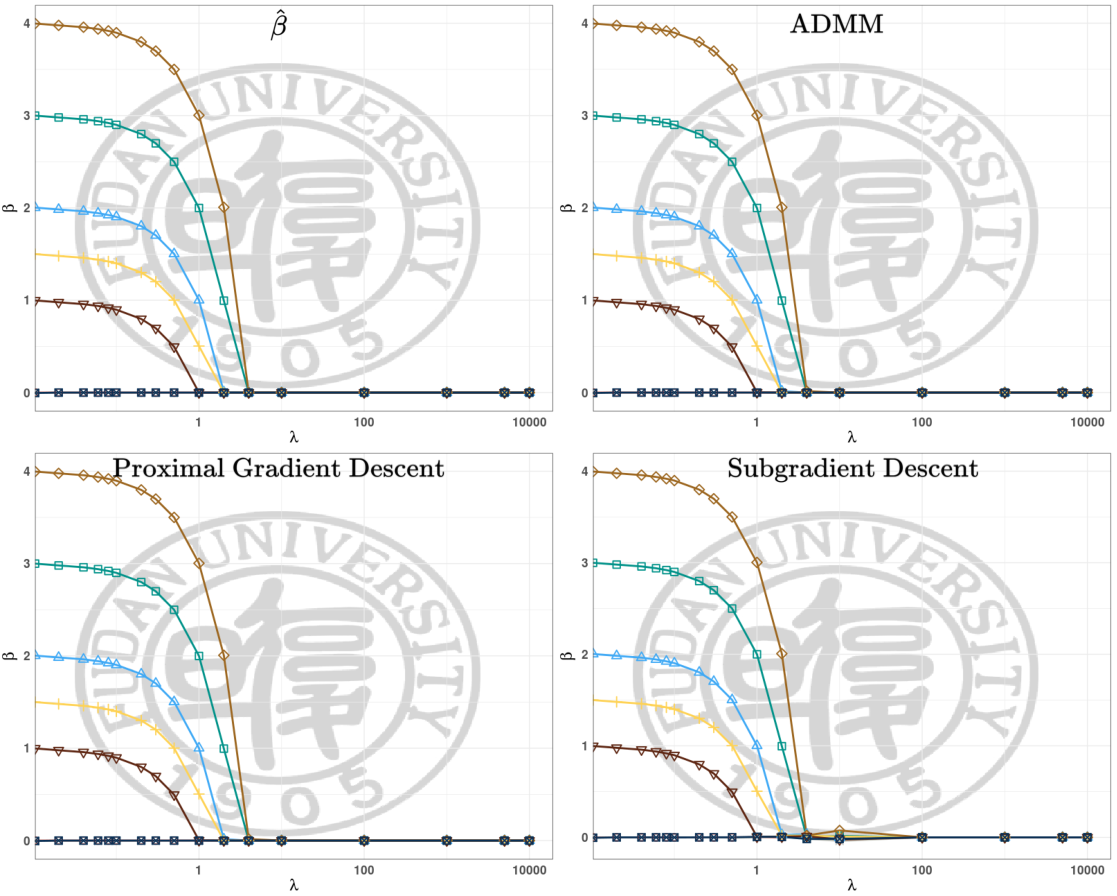
\includegraphics[width=0.8\textwidth]{image/scenario1}
        \caption{The estimation of $\beta$ using four different algorithms}
        \label{fig:shrinkage_para}
    \end{figure}
\end{center}
As shown in Figure \ref{fig:shrinkage_para}, all estimation values of $\beta$ converges to zero as $\lambda$ grows. Besides, we can see the global estimator $\tilde{\beta}$ obtained by the distributed algorithm (i.e., Algorithm \ref{algo:dlr}) is very closed to the global estimator $\widehat{\beta}$ on the whole dataset, which means our algorithm is accurate and effective. 

\noindent
{\sc \textbf{Scenario 2 (Sample Size)}}
In this scenario, we observe how the $\operatorname{RMSE}$ changes with respect to the sample size. Accordingly we fix $K=5$, $\lambda=0.001$ and vary the sample size from 500 to 10000. In the meanwhile, we set the $\beta_0 = (3, 2, 1.5, 4, 1)^{\top}$ and the method we used on worker is \textbf{Proximal Gradient Descent}. The result is summarized in  Figure \ref{fig:effet_of_N}.
\vspace{-0.5cm}
\begin{center}
    \begin{figure}[h]
        \centering
        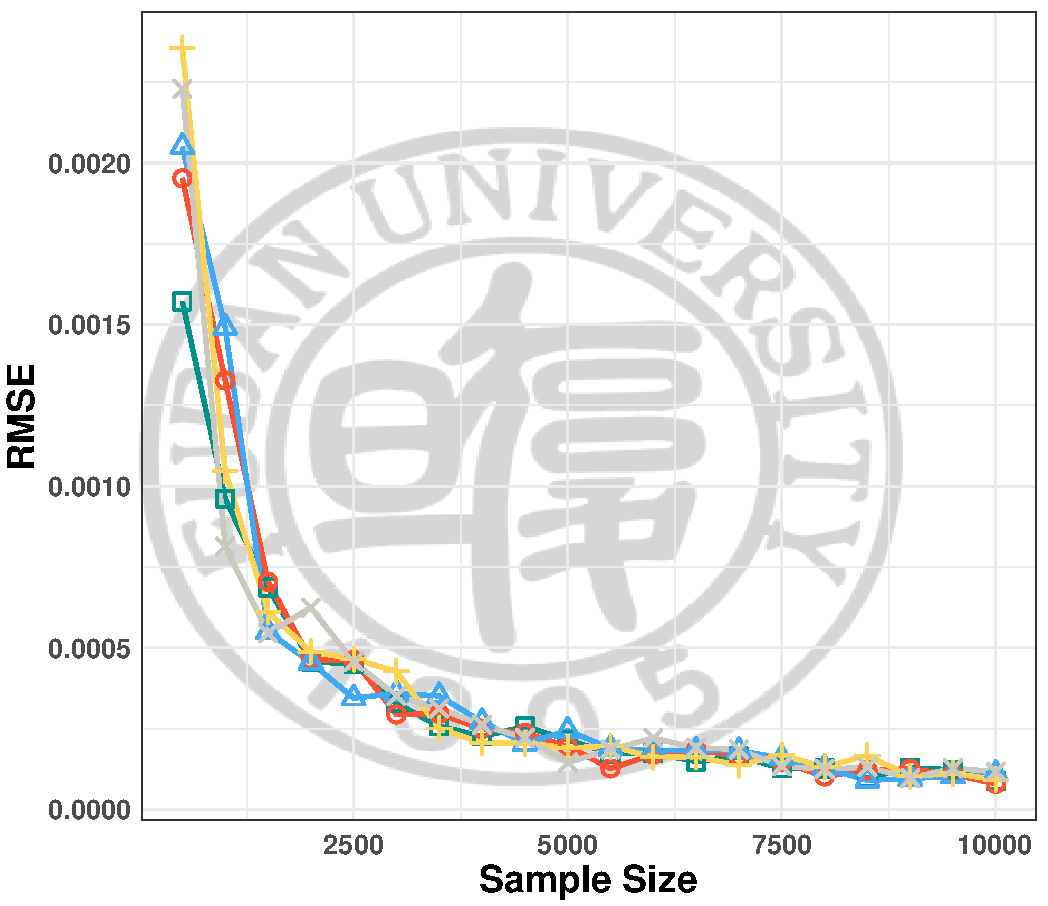
\includegraphics[width=0.5\textwidth]{image/scenario2}
        \caption{$\operatorname{RMSE}$ of each dimension in $\beta$ under different $N$}
        \label{fig:effet_of_N}
    \end{figure}
\end{center}
As shown in Figure \ref{fig:effet_of_N}, the $\operatorname{RMSE}$ converges to zero as the sample size grows, which corroborates with our theoretical findings in Theorem \ref{theorem:global}. Besides, we can see the converge rate is very fast, when the sample size equals to 8000 (i.e. each worker has 1600 points), the $\operatorname{RMSE}$ is less than $10^{-4}$.

\noindent
{\sc \textbf{Scenario 3 (Worker Number)}}
In this setting, we verify the worker number effect on the finite sample performances. First, we fix $N = 1000$, $\lambda = 0.001$. Then, we set the $\beta_0 = (3, 2, 1.5, 4, 1)^{\top}$ and vary $K$ from 5 to 100. As the same in Scenario 2, we use \textbf{Proximal Gradient Descent} on each worker to get $\hat{\beta}_k$. The result is summarized in  Figure \ref{fig:effet_of_K}.
\vspace{-0.5cm}
\begin{center}
    \begin{figure}[h]
        \centering
        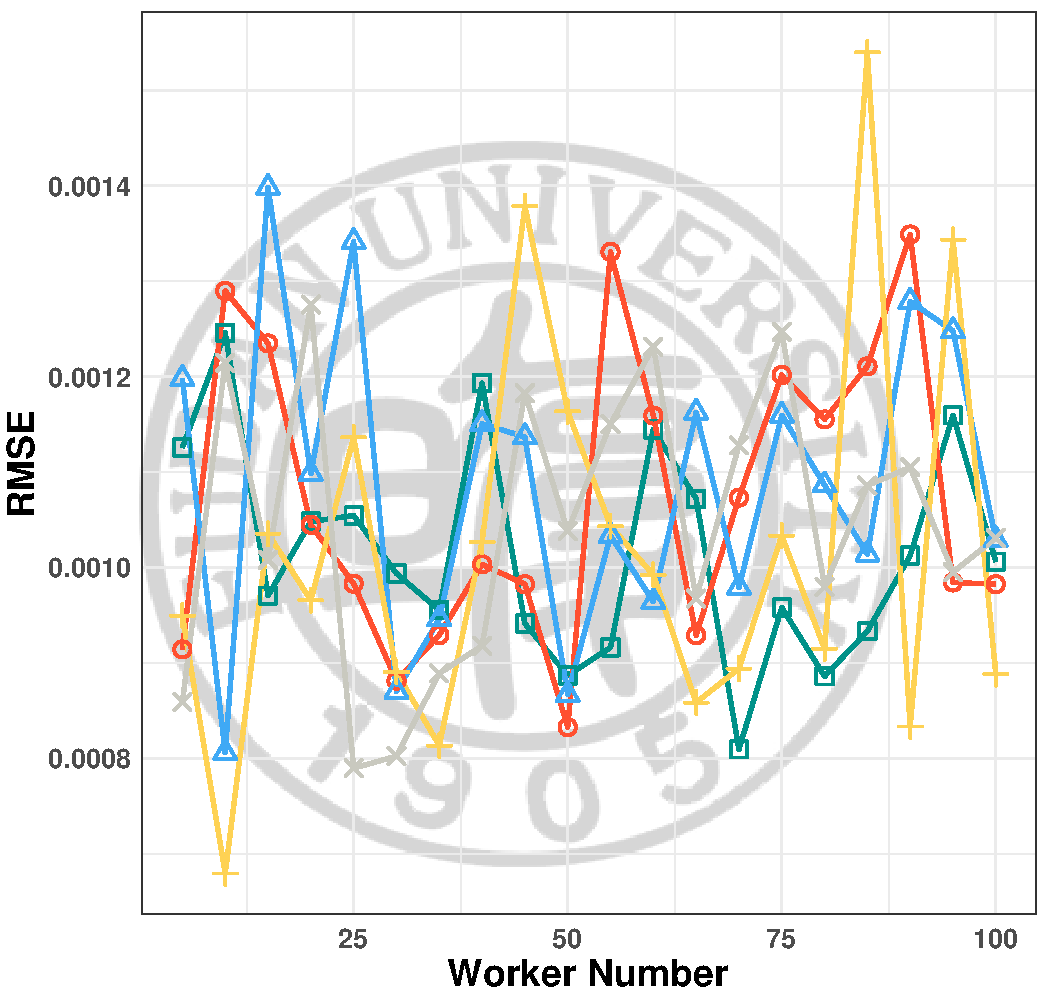
\includegraphics[width=0.4\textwidth]{image/scenario3}
        \caption{$\operatorname{RMSE}$ of each dimension in $\beta$ under different $K$}
        \label{fig:effet_of_K}
    \end{figure}
\end{center}
As shown in Figure \ref{fig:effet_of_K}, worker number has no effect on the $\operatorname{RMSE}$. This is because each worker contributes the weight $\alpha_k \hat{\Sigma}_k^{-1}$, which makes the global estimator $\tilde{\beta}$ consistent even if the sample size on each worker is small. Therefore, even if there are many workers in the distributed system, our algorithm could still get the  consistent global estimator $\tilde{\beta}$. However, the effect of worker number needs to explore in the further study.

\section{APPLICATION TO USEDCAR DATA}\label{sec:5}

\subsection{Data Description}

For illustration purposes, we study a real-world dataset. Specifically, the dataset is the U.S. USERCAR Dataset, which is available at \href{tianchi.aliyun.com}{tianchi.aliyun.com}. It contains detailed used car trading information from a website. The task is to predict the price of the used car with a regression model. Each sample in the data corresponds to one used car record, which consists of many variables such as "fuel tpye", "seller", "price". The complete variable information is described in Table .The total sample size is 150 thousand observations.

\subsection{The Spark System}

To demonstrate our method, we set up a Spark-on-YARN cluster on three servers . This is a standard industrial-level architecture setup for a distributed system. The system consists of one master node and two worker nodes. Each node contains 32 virtual cores, 64 GB of RAM. The dataset is stored on the Hadoop data file system (HDFS).

\subsection{The DLR Method}

For the USEDCAR dataset, we perform our DLR algorithm on the Spark and finally get the results. Besides, we compare our result with the solver in \textbf{"sklearn"} package of \textbf{Python} and the result is summarized as Table 1 in Appendix. We can see that there is a big difference between the traditional method in \textbf{"sklearn"} package with our DLR method. This is due to the bad initial value, how to get a good initial value is an interesting problem and it will be discussed in the further study.

\section{CONCLUDING REMARKS}\label{sec:6}

In this work, we propose a distributed lasso regression (DLR) algorithm to tackle regression task in large dataset. The proposed DLR algorithm has three merits. First, the communication cost is low since it requires only one round of communication. Second, no further iterative algorithm is needed on master and hence it does not suffer from problems as initialization and non-robustness. Third, the computational complexity is much lower compared to get the global estimator using whole dataset. 

To conclude the article, we provide several topics for future studies. First, better mechanisms can be designed to get a better initial point. This enables us to obtain more accurate estimation of the pseudo centers and yields better clustering results. Next, it is interesting to discuss the effect of the worker number. Third, it is important to explore how to reduce the iterations of the algorithm on each worker.

\section*{Acknowledgment}\label{acknowledgment}
\addcontentsline{toc}{section}{Acknowledgment}

Thanks to Prof. Jiang for his teaching and guidance over the past semester. As a student of school of big data, this course gives us a very intuitive understanding of optimization algorithm. I believe the knowledge of this course will be of great help to our future research. At the same time,I would like to thank all the teaching assistants for correcting ours homework carefully and patiently answering our various questions, which has greatly helped our study of this course.

\newpage

\section*{Appendix: Result of U.S. USERCAR Dataset}\label{appendix}
\addcontentsline{toc}{section}{Appendix: Result of U.S. USERCAR Dataset}

\begin{table}[h]
\label{table_res}
\centering
\begin{tabular}{c||c|c|c|c}
\hline
\hline
\textbf{Variable Number} & \textbf{Sklearn} &  \textbf{PGM}    &   \textbf{ADMM} &  \textbf{Sub-GD} \\ 
 \hline
1 & 0.0000  & -0.0094 &  0.0000 & -0.0094 \\ 
2 & 0.0797  & -0.0813 &  0.0794 &  0.0813 \\
3 & -0.0086 & -0.0058 & -0.0090 & -0.0058 \\
4 & 0.0647  &  0.0622 &  0.0645 &  0.0622 \\
5 & 0.0000  & -0.0001 & -0.0004 & -0.0001 \\
6 & 0.0776  &  0.0756 &  0.0773 &  0.0756 \\
7 & 0.0517  &  0.0579 &  0.0580 &  0.0579 \\
8 & -0.1813 & -0.1832 & -0.1812 & -0.1832 \\
9 & 0.0039  &  0.0047 &  0.0044 &  0.0047 \\
10 & 0.0112  &  0.0119 &  0.0111 &  0.0119 \\
11 & 0.0011  &  0.0007 &  0.0006 &  0.0007 \\
12 & 0.0077  &  0.0076 &  0.0077 &  0.0076 \\
13 & 0.1259  &  0.3123 &  0.1260 &  0.3122 \\
14 & 0.0000  &  0.0004 &  0.0000 &  0.0004 \\
15 & 0.0058  &  0.0711 &  0.0000 &  0.0711 \\
16 & 0.0000  & -0.0362 &  0.0000 & -0.0362 \\
17 & -0.1849 & -0.1063 & -0.1875 & -0.1063 \\
18 & 0.0000  &  0.0000 &  0.0000 &  0.0000 \\
19 & 0.2311  &  0.0317 &  0.2261 &  0.0318 \\
20 & 0.0000  &  0.0000 &  0.0000 &  0.0000 \\
21 & 0.5992  &  0.2205 &  0.5791 &  0.2205 \\
22 & 0.5056  &  0.2258 &  0.5017 &  0.2258 \\
23 & 0.0000  & -0.0045 &  0.0000 & -0.0455 \\
24 & 0.0000  &  0.0000 &  0.0000 &  0.0000 \\
25 & 0.1418  &  0.2473 &  0.1597 &  0.2473 \\
26 & -0.4704 & -0.1811 & -0.4592 & -0.1811 \\
27 & 0.1414  &  0.1138 &  0.1403 &  0.1138 \\
28 & 0.0121  &  0.0098 &  0.0118 &  0.0098 \\
\hline
\end{tabular}
\caption{Coefficients for the logistic model estimated with three different DLR method (PGM, ADMM, Sub-GD) and the method in \textbf{"sklearn"} package}
\end{table}

\newpage

\bibliographystyle{asa}
\bibliography{reference}
\addcontentsline{toc}{section}{References}

\end{document}
